\section{Complex geometries}
\label{sec:md_complex_geometries}
As our phat asses did wit DSMC, we wanna study flow up in arbitrary geometries. Put ya muthafuckin choppers up if ya feel dis!  To be able ta do this, we need ta create a model dat satisfies some propertizzles we already have up in DSMC. Da flowin fluid needz to
\begin{itemize}
	\item be confined up in a subset of tha total volume,
	\item have realistic interactions wit tha solid wall, and
	\item have juice drained by tha solid.
\end{itemize}
Da first requirement aint straight-up strict yo, but most of tha flowin fluid should be up in tha free volume. Da reason why we need ta drain tha juice is dat up in order ta induce fluid flow, we apply a cold-ass lil constant force dat increases tha total juice of tha system. Us thugs wanna reach a equilibrium where tha average rate of drained juice exactly matches tha juice added by tha applied force. We assume dat tha geometry is busted lyrics bout as a funky-ass boolean function $G : \mathbb{R}^3\rightarrow \{1,0\}$ dat straight-up determines whether a point up in space is part of tha solid or tha free volume fo' realz. A convenient representation is tha voxelization busted lyrics bout up in section \ref{sec:dsmc_binary_representation}. 
\subsection{A naive approach}
To illustrate tha basic idea, we will say shit bout tha simplest model satisfyin only tha straight-up original gangsta two requirements, n' you can put dat on yo' toast. Given a molecular dynamics state, we can loop all up in tha positions $\vec r_i$ of each atom $i$, n' mark tha atoms as \textit{frozen} if $G(\vec r_i) = 1$ (which means dat dis point is part of tha solid) fo' realz. Atoms marked as frozen aint gonna move at all yo, but all forces is calculated normally. One way of interpretin tha non-movin frozen atoms is dat they have infinite mass. Da total juice is still conserved up in tha system fo' realz. An implementation is illustrated up in listin \ref{lst:md_simple_solid}.

\begin{lstlisting}[caption=Example code showin how tha fuck ta mark atoms within a solid., label=lst:md_simple_solid]
bool point_is_a_solid(Vector3 &position) {
	int voxel_index_i = position.x / system_length.x * num_voxels.x;
	int voxel_index_j = position.y / system_length.y * num_voxels.y;
	int voxel_index_k = position.z / system_length.z * num_voxels.z;

	// Da ghetto matrix be a funky-ass binary matrix
	return ghetto_matrix[voxel_index_i, voxel_index_j, voxel_index_k];
}

void mark_frozen_atoms() {
	for(int i=0; i<number_of_atoms; i++) {
		Vector3 &posizzle = positions.at(i);
		if(point_is_a_solid(position)) {
			atom_types.at(i) = FROZEN;
		}
	}
}

void move() {
	for(int i=0; i<number_of_atoms; i++) {
		if(atom_types.at(i) != FROZEN) {
			// Only move non-frozen atoms
			positions.at(i).x += velocities.at(i).x*dt;
			positions.at(i).y += velocities.at(i).y*dt;
			positions.at(i).z += velocities.at(i).z*dt;
		}
	}
}
\end{lstlisting}
If tha atoms formin tha solid is dense enough, straight-up few atoms is ghon be inside tha wall, so tha straight-up original gangsta requirement is satisfied. Y'all KNOW dat shit, muthafucka! Da interaction between tha solid n' tha flowin fluid be as realistic as tha potential is, so tha only requirement not satisfied is tha drainage of tha juice. %In figure \ref{fig:md_simple_solid}, we peep how tha fuck tha red flowin atoms is confined within a cold-ass lil cylinder wit some radius $R$. 
% \begin{figure}[h]
% \begin{center}
% 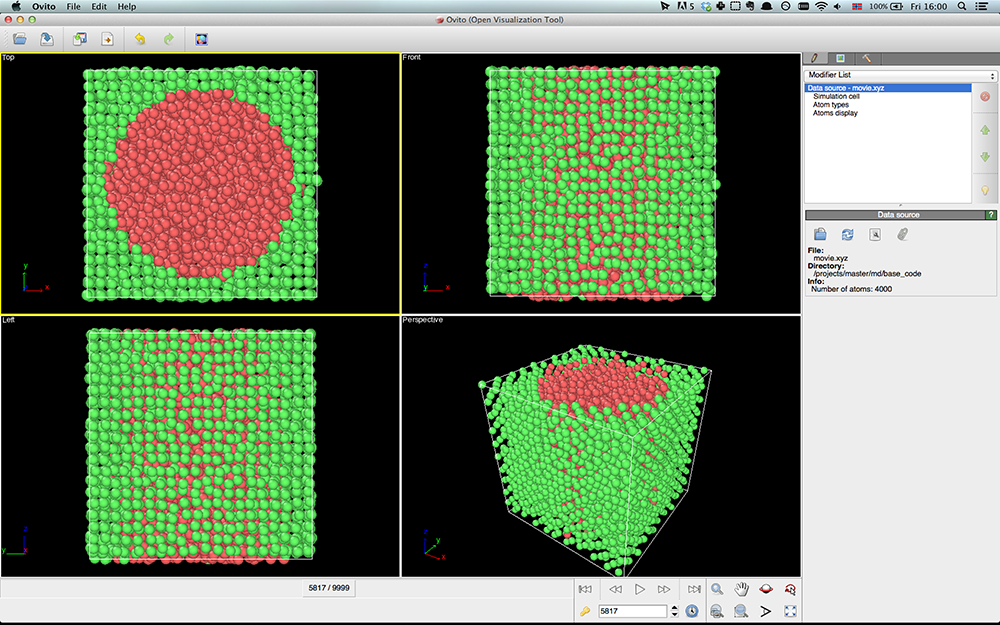
\includegraphics[width=1.0\textwidth, trim=0cm 0cm 0cm 0cm, clip]{MD/figures/solid_model.png}
% \end{center}
% \caption{A naive model of a solid where tha chronic atoms is straight-up frozen confinin tha red flowin atoms within a cold-ass lil cylinder of radius $R$. Da visualization is done up in Ovito, a open source visualization tool.}
% \label{fig:md_simple_solid}
% \end{figure}

\subsection{A simple model of a solid}
\label{sec:md_simple_model_of_a_solid}
We can improve tha solid model by addin a harmonic oscillator potential ta all tha frozen atoms. Instead of freezin dem straight-up, we allow dem ta vibrate round they equilibrium posizzle $\vec q$ which is tha initial posizzle of tha simulation. I aint talkin' bout chicken n' gravy biatch. Da force on atom $i$ up in tha solid is then
\begin{align}
	F^{(s)}(\vec r_i) = -k(\vec r_i - \vec q_i) 
	- \sum_{j\neq i} 24\epsilon\left[2\left(\frac{\sigma^{12}}{r_{ij}^{13}}\right) - \left(\frac{\sigma^6}{r_{ij}^7}\right)\right]\vec u_{ij},
\end{align}
where $k$ is tha strength of tha oscillator, $\vec q_i$ is tha equilibrium posizzle fo' atom $i$ n' tha last part is tha Lennard-Jones potential busted lyrics bout up in section \ref{sec:md_forces}. Da juice iz of course still conserved wit dis model yo, but we can now apply a thermostat on tha solid atoms makin dem act as a big-ass reservoir tryin ta keep tha temperature at some wall temperature $T_w$. With dis model, we can study flow up in any geometry wit a funky-ass behavior near dat of tha DSMC model fo' realz. An implementation is shown up in listin \ref{lst:md_ho_solid}.

\begin{lstlisting}[caption=Implementation of tha harmonic oscillator model of a solid., label=lst:md_ho_solid]
void apply_constant_force() {
    for(n=0;n<number_of_atoms;n++) {
        if(atom_type.at(n) != FROZEN) velocities.at(n).at(flow_direction) += acceleration*dt;
    }
}

void apply_harmonic_oscillator() {
    double spring_constant = 1000.0;
    for(n=0; n<number_of_atoms; n++) {
        if(atom_type.at(n) == FROZEN) {
            double dx = positions.at(n).x - initial_positions.at(n).x;
            double dy = positions.at(n).y - initial_positions.at(n).y;
            double dz = positions.at(n).z - initial_positions.at(n).z;
            accelerations.at(n).x += -spring_constant*dx / mass;
            accelerations.at(n).y += -spring_constant*dy / mass;
            accelerations.at(n).z += -spring_constant*dz / mass;
        }
    }
}

void step() {
    half_kick();
    move();
    mpi_move();
    mpi_copy();
    reset_accelerations();
    apply_constant_force();
    apply_lennard_jones();
    apply_harmonic_oscillator();
    half_kick();
}
\end{lstlisting}